% Convolution of two rectangular bumps: indicators of [0,1] and [0,2], and the trapezoid they produce.
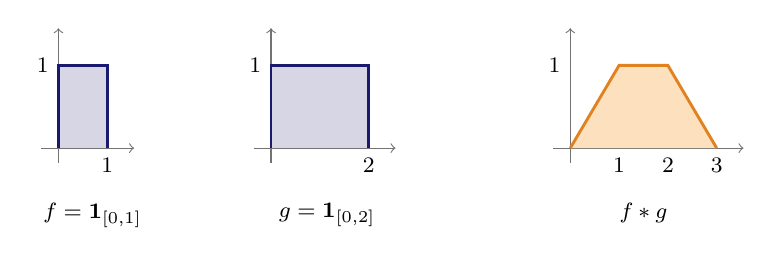
\begin{tikzpicture}[x=0.62cm,y=1.05cm,every node/.style={font=\footnotesize}]
  % f = indicator of [0,1]
  \begin{scope}
    \draw[->,black!55] (-0.35,0) -- (1.55,0);
    \draw[->,black!55] (0,-0.18) -- (0,1.45);
    \fill[MidnightBlue!18] (0,0) rectangle (1,1);
    \draw[MidnightBlue,line width=1.05pt] (0,0) -- (0,1) -- (1,1) -- (1,0);
    \node[below] at (1,0) {$1$};
    \node[left] at (0,1) {$1$};
    \node[anchor=north] at (0.7,-0.55) {$f=\mathbf{1}_{[0,1]}$};
  \end{scope}
  % g = indicator of [0,2]
  \begin{scope}[xshift=2.7cm]
    \draw[->,black!55] (-0.35,0) -- (2.55,0);
    \draw[->,black!55] (0,-0.18) -- (0,1.45);
    \fill[MidnightBlue!18] (0,0) rectangle (2,1);
    \draw[MidnightBlue,line width=1.05pt] (0,0) -- (0,1) -- (2,1) -- (2,0);
    \node[below] at (2,0) {$2$};
    \node[left] at (0,1) {$1$};
    \node[anchor=north] at (1.15,-0.55) {$g=\mathbf{1}_{[0,2]}$};
  \end{scope}
  % f*g, the trapezoid of height 1 on [0,3]
  \begin{scope}[xshift=6.5cm]
    \draw[->,black!55] (-0.35,0) -- (3.55,0);
    \draw[->,black!55] (0,-0.18) -- (0,1.45);
    \fill[BurntOrange!22] (0,0) -- (1,1) -- (2,1) -- (3,0) -- cycle;
    \draw[BurntOrange!90!black,line width=1.05pt] (0,0) -- (1,1) -- (2,1) -- (3,0);
    \node[below] at (1,0) {$1$};
    \node[below] at (2,0) {$2$};
    \node[below] at (3,0) {$3$};
    \node[left] at (0,1) {$1$};
    \node[anchor=north] at (1.5,-0.55) {$f*g$};
  \end{scope}
\end{tikzpicture}
